\chapter{Background}
\label{chap:Background}
In this chapter the subjects needed to comprehend the rest of the thesis will be discussed. The most common subjects will be ignored, giving a focus on the more specific and less common ones.

\section{Burp Suite community edition}
Burp Suite Community Edition (from now on \Gls{burp}) is one of the most used application security testing software for web security testing. It works by the use of a proxy server over which a browser redirects the traffic to. The proxy does like a Man In The Middle attack, taking the input traffic from the browser and replying the HTTP messages (from now on messages) to the target service, giving also transparency over the TSL (Transport Layer Security) or SSL (Secure Socket Layer) encryption. \Gls{burp} has access to the proxy, it can sniff HTTP packets and can edit them before they are forwarded to the browser or the target service. \Gls{burp} also gives the possibility of creating custom plugins giving to the developers access to the java API. This is exactly how the plugin (from now on tool) will be implemented, using \Gls{burp} as a base over which develop the software that will execute the tests. The tool will be able to intercept, read and edit messages that pass through the \Gls{burp}'s proxy by the use of \Gls{burp}'s API.

\section{JSON}
As stated in \cite{json_standard}: "JavaScript Object Notation (JSON) is a text format for the serialization of structured data.  It is derived from the object literals of JavaScript. JSON can represent four primitive types (strings, numbers, booleans, and null) and two structured types (objects and arrays). An object is an unordered collection of zero or more name/value pairs, where a name is a string and a value is a string, number, boolean, null, object, or array. An array is an ordered sequence of zero or more values".
In this thesis, the word "name" identifying a name/value pairs, will not be used and will be substituted with "tag".

\section{Regex}
Regex stands for regular expression, it is a sequence of symbols that define an ensemble of strings that can be matched by it. There is a list of symbols that can be used to specify which characters to match. For example, if the value of the "Host" header in a message has to be found, a regex like this one has to be defined: \verb|Host:\s?.*|
This regex will search for the string "Host:" followed by 0 or 1 whitespace, and all the characters that follow until "\verb|\n|" is found. This is a complete explanation of the symbols used in this example:
\begin{itemize}
    \item \verb|\s| is the whitespace character
    \item \textbf{?} is an operator that tells that the preceding symbol will be matched 0 or 1 times
    \item \textbf{*} is an operator that tells that the preceding symbol will be matched 0 or more times
    \item \textbf{.} matches any character except line breaks
\end{itemize}

\section{IdM protocols: SAML and OAuth}
Identity Management (IdM) protocols are protocols that deals with identity management. For the aim of this thesis, \gls{SAML} (Security Assertion Markup Language) and \gls{OAuth} 2.0 (from now on \gls{OAuth}) will be discussed, as they are used in the examples and in related works.
\begin{wrapfigure}{r}{0.5\textwidth}
    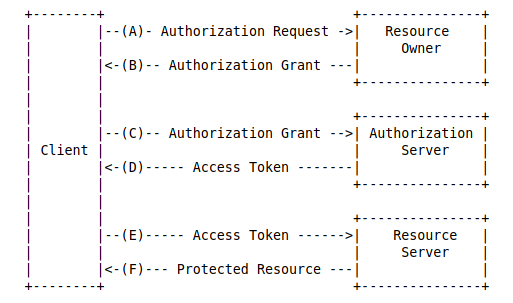
\includegraphics[width=0.9\linewidth]{OAuth_protocol_flow.png}
    \caption{OAuth abstract protocol flow\\source \cite{ietf_oauth2}}
    \label{fig:OAuth_protocol_flow}
\end{wrapfigure}
Both \Gls{SAML} and \gls{OAuth} are Single Sign-On (SSO) protocols, they follow an authentication scheme that allows a user to log in with a single ID and password to any of several related, yet independent, software systems, a more complete explanation can be found in \cite{claudio_grisenti}. 
The difference between \Gls{SAML} and \gls{OAuth} is how they work, but their objective is the same: to certificate the identity of a given person in different circumstances.

\subsection{OAuth}
As stated in \cite{ietf_oauth2}, the \gls{OAuth} authorization framework enables a third-party application to obtain limited access to an HTTP service, either on behalf of a resource owner by orchestrating an approval interaction between the resource owner and the HTTP service, or by allowing the third-party application to obtain access on its own behalf.
A series of messages has to be exchanged between the two parties in order to authenticate a resource owner that wants to access some reserved data in a service. As described in \cite{ietf_oauth2}, the flow illustrated in \ref{fig:OAuth_protocol_flow} describes the interaction between the four roles and includes the following steps:
\begin{enumerate}[(A)]
    \item The client requests authorization from the resource owner.  The authorization request can be made directly to the resource owner (as shown), or preferably indirectly via the authorization server as an intermediary.
    \item The client receives an authorization grant, which is a credential representing the resource owner's authorization, expressed using one of four grant types defined in this specification or using an extension grant type. The authorization grant type depends on the method used by the client to request authorization and the types supported by the authorization server.
    \item The client requests an access token by authenticating with the authorization server and presenting the authorization grant.
    \item The authorization server authenticates the client and validates the authorization grant, and if valid, issues an access token.
    \item The client requests the protected resource from the resource server and authenticates by presenting the access token.
    \item The resource server validates the access token, and if valid, serves the request.
\end{enumerate}
 
\subsubsection{PKCE}
As stated in \cite{pkce_downgrade}: OAuth 2.0 public clients utilizing the Authorization Code Grant are susceptible to the authorization code interception attack. A technique to mitigate against the threat is the use of Proof Key for Code Exchange (PKCE, pronounced "pixy"). The PKCE extension utilizes a dynamically created cryptographically random key called "code verifier".  A unique code verifier is created for every authorization request, and its transformed value, called "code challenge", is sent to the authorization server to obtain the authorization code.  The authorization code obtained is then sent to the token endpoint with the "code verifier", and the server compares it with the previously received request code so that it can perform the proof of possession of the "code verifier" by the client.  This works as the mitigation since the attacker would not know this one-time key, since it is sent over TLS and cannot be intercepted.
The PKCE specification adds additional parameters to the OAuth 2.0 Authorization and Access Token Requests:
\begin{enumerate}[(A)]
    \item The client creates and records a secret named the "code\_verifier" and derives a transformed version "t(code\_verifier)" (referred to as the "code\_challenge"), which is sent in the OAuth 2.0 Authorization Request along with the transformation method "t\_m". 
    \item The Authorization Endpoint responds as usual but records "t(code\_verifier)" and the transformation method. 
    \item The client then sends the authorization code in the Access Token Request as usual but includes the "code\_verifier" secret generated at (A). 
    \item The authorization server transforms "code\_verifier" and compares it to "t(code\_verifier)" from (B).  Access is denied if they are not equal.
\end{enumerate}
An attacker who intercepts the authorization code at (B) is unable to redeem it for an access token, as they are not in possession of the "code\_verifier" secret.

\subsection{SAML - Security Assertion Markup Language}
As stated in \cite{ietf_SAML}, "The Security Assertion Markup Language (\Gls{SAML}) 2.0 is an XML-based framework that allows identity and security information to be shared across security domains. The Assertion, an XML security token, is a fundamental construct of \Gls{SAML} that is often adopted for use in other protocols and specifications. An Assertion is generally issued by an Identity Provider and consumed by a Service Provider that relies on its content to identify the Assertion's subject for security-related purposes."





